\documentclass[twoside]{book}

% Packages required by doxygen
\usepackage{fixltx2e}
\usepackage{calc}
\usepackage{doxygen}
\usepackage[export]{adjustbox} % also loads graphicx
\usepackage{graphicx}
\usepackage[utf8]{inputenc}
\usepackage{makeidx}
\usepackage{multicol}
\usepackage{multirow}
\PassOptionsToPackage{warn}{textcomp}
\usepackage{textcomp}
\usepackage[nointegrals]{wasysym}
\usepackage[table]{xcolor}

% Font selection
\usepackage[T1]{fontenc}
\usepackage[scaled=.90]{helvet}
\usepackage{courier}
\usepackage{amssymb}
\usepackage{sectsty}
\renewcommand{\familydefault}{\sfdefault}
\allsectionsfont{%
  \fontseries{bc}\selectfont%
  \color{darkgray}%
}
\renewcommand{\DoxyLabelFont}{%
  \fontseries{bc}\selectfont%
  \color{darkgray}%
}
\newcommand{\+}{\discretionary{\mbox{\scriptsize$\hookleftarrow$}}{}{}}

% Page & text layout
\usepackage{geometry}
\geometry{%
  a4paper,%
  top=2.5cm,%
  bottom=2.5cm,%
  left=2.5cm,%
  right=2.5cm%
}
\tolerance=750
\hfuzz=15pt
\hbadness=750
\setlength{\emergencystretch}{15pt}
\setlength{\parindent}{0cm}
\setlength{\parskip}{3ex plus 2ex minus 2ex}
\makeatletter
\renewcommand{\paragraph}{%
  \@startsection{paragraph}{4}{0ex}{-1.0ex}{1.0ex}{%
    \normalfont\normalsize\bfseries\SS@parafont%
  }%
}
\renewcommand{\subparagraph}{%
  \@startsection{subparagraph}{5}{0ex}{-1.0ex}{1.0ex}{%
    \normalfont\normalsize\bfseries\SS@subparafont%
  }%
}
\makeatother

% Headers & footers
\usepackage{fancyhdr}
\pagestyle{fancyplain}
\fancyhead[LE]{\fancyplain{}{\bfseries\thepage}}
\fancyhead[CE]{\fancyplain{}{}}
\fancyhead[RE]{\fancyplain{}{\bfseries\leftmark}}
\fancyhead[LO]{\fancyplain{}{\bfseries\rightmark}}
\fancyhead[CO]{\fancyplain{}{}}
\fancyhead[RO]{\fancyplain{}{\bfseries\thepage}}
\fancyfoot[LE]{\fancyplain{}{}}
\fancyfoot[CE]{\fancyplain{}{}}
\fancyfoot[RE]{\fancyplain{}{\bfseries\scriptsize Generated by Doxygen }}
\fancyfoot[LO]{\fancyplain{}{\bfseries\scriptsize Generated by Doxygen }}
\fancyfoot[CO]{\fancyplain{}{}}
\fancyfoot[RO]{\fancyplain{}{}}
\renewcommand{\footrulewidth}{0.4pt}
\renewcommand{\chaptermark}[1]{%
  \markboth{#1}{}%
}
\renewcommand{\sectionmark}[1]{%
  \markright{\thesection\ #1}%
}

% Indices & bibliography
\usepackage{natbib}
\usepackage[titles]{tocloft}
\setcounter{tocdepth}{3}
\setcounter{secnumdepth}{5}
\makeindex

% Hyperlinks (required, but should be loaded last)
\usepackage{ifpdf}
\ifpdf
  \usepackage[pdftex,pagebackref=true]{hyperref}
\else
  \usepackage[ps2pdf,pagebackref=true]{hyperref}
\fi
\hypersetup{%
  colorlinks=true,%
  linkcolor=blue,%
  citecolor=blue,%
  unicode%
}

% Custom commands
\newcommand{\clearemptydoublepage}{%
  \newpage{\pagestyle{empty}\cleardoublepage}%
}

\usepackage{caption}
\captionsetup{labelsep=space,justification=centering,font={bf},singlelinecheck=off,skip=4pt,position=top}

%===== C O N T E N T S =====

\begin{document}

% Titlepage & ToC
\hypersetup{pageanchor=false,
             bookmarksnumbered=true,
             pdfencoding=unicode
            }
\pagenumbering{alph}
\begin{titlepage}
\vspace*{7cm}
\begin{center}%
{\Large My Project }\\
\vspace*{1cm}
{\large Generated by Doxygen 1.8.13}\\
\end{center}
\end{titlepage}
\clearemptydoublepage
\pagenumbering{roman}
\tableofcontents
\clearemptydoublepage
\pagenumbering{arabic}
\hypersetup{pageanchor=true}

%--- Begin generated contents ---
\chapter{Hierarchical Index}
\section{Class Hierarchy}
This inheritance list is sorted roughly, but not completely, alphabetically\+:\begin{DoxyCompactList}
\item \contentsline{section}{vocabulary}{\pageref{classvocabulary}}{}
\begin{DoxyCompactList}
\item \contentsline{section}{admin}{\pageref{classadmin}}{}
\item \contentsline{section}{user}{\pageref{classuser}}{}
\end{DoxyCompactList}
\end{DoxyCompactList}

\chapter{Class Index}
\section{Class List}
Here are the classes, structs, unions and interfaces with brief descriptions\+:\begin{DoxyCompactList}
\item\contentsline{section}{\hyperlink{classadmin}{admin} }{\pageref{classadmin}}{}
\item\contentsline{section}{\hyperlink{classuser}{user} }{\pageref{classuser}}{}
\item\contentsline{section}{\hyperlink{classvocabulary}{vocabulary} }{\pageref{classvocabulary}}{}
\end{DoxyCompactList}

\chapter{Class Documentation}
\hypertarget{classadmin}{}\section{admin Class Reference}
\label{classadmin}\index{admin@{admin}}


Inheritance diagram for admin\+:\nopagebreak
\begin{figure}[H]
\begin{center}
\leavevmode
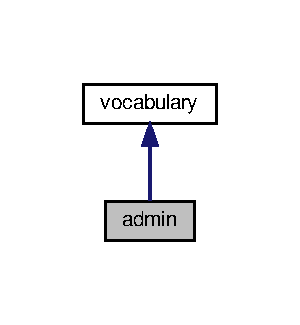
\includegraphics[width=144pt]{classadmin__inherit__graph}
\end{center}
\end{figure}


Collaboration diagram for admin\+:\nopagebreak
\begin{figure}[H]
\begin{center}
\leavevmode
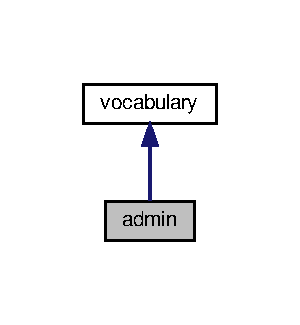
\includegraphics[width=144pt]{classadmin__coll__graph}
\end{center}
\end{figure}
\subsection*{Public Member Functions}
\begin{DoxyCompactItemize}
\item 
\mbox{\Hypertarget{classadmin_a39d5c1977388ccd1c5816cd1586a7d22}\label{classadmin_a39d5c1977388ccd1c5816cd1586a7d22}} 
void {\bfseries adminmenu} ()
\item 
\mbox{\Hypertarget{classadmin_aa0f88152929ea72f713d9fe30f4661ca}\label{classadmin_aa0f88152929ea72f713d9fe30f4661ca}} 
void {\bfseries add} ()
\item 
\mbox{\Hypertarget{classadmin_a49bb00bce0e4aa6be4611cd650e034b3}\label{classadmin_a49bb00bce0e4aa6be4611cd650e034b3}} 
void {\bfseries delete\+\_\+word} ()
\item 
\mbox{\Hypertarget{classadmin_a33d43e29829005a9f46c581a981a9f0b}\label{classadmin_a33d43e29829005a9f46c581a981a9f0b}} 
void {\bfseries modify\+\_\+meaning} ()
\end{DoxyCompactItemize}
\subsection*{Additional Inherited Members}


The documentation for this class was generated from the following files\+:\begin{DoxyCompactItemize}
\item 
header.\+h\item 
admin.\+h\end{DoxyCompactItemize}

\hypertarget{classuser}{}\section{user Class Reference}
\label{classuser}\index{user@{user}}


Inheritance diagram for user\+:\nopagebreak
\begin{figure}[H]
\begin{center}
\leavevmode
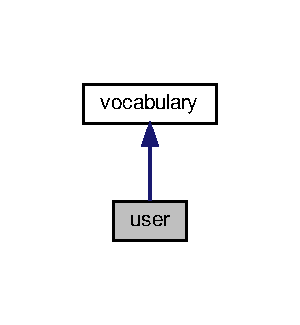
\includegraphics[width=144pt]{classuser__inherit__graph}
\end{center}
\end{figure}


Collaboration diagram for user\+:\nopagebreak
\begin{figure}[H]
\begin{center}
\leavevmode
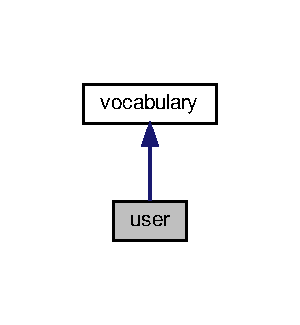
\includegraphics[width=144pt]{classuser__coll__graph}
\end{center}
\end{figure}
\subsection*{Public Member Functions}
\begin{DoxyCompactItemize}
\item 
\mbox{\Hypertarget{classuser_a18767ad955443aa3cd2f60256e973a76}\label{classuser_a18767ad955443aa3cd2f60256e973a76}} 
void {\bfseries usermenu} ()
\end{DoxyCompactItemize}
\subsection*{Additional Inherited Members}


The documentation for this class was generated from the following files\+:\begin{DoxyCompactItemize}
\item 
header.\+h\item 
user.\+h\end{DoxyCompactItemize}

\hypertarget{classvocabulary}{}\section{vocabulary Class Reference}
\label{classvocabulary}\index{vocabulary@{vocabulary}}


Inheritance diagram for vocabulary\+:\nopagebreak
\begin{figure}[H]
\begin{center}
\leavevmode
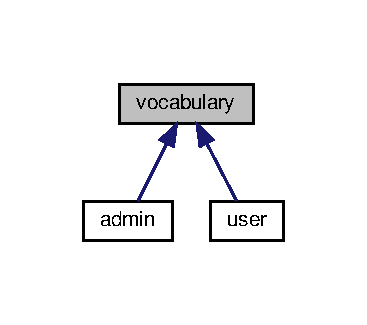
\includegraphics[width=176pt]{classvocabulary__inherit__graph}
\end{center}
\end{figure}
\subsection*{Public Member Functions}
\begin{DoxyCompactItemize}
\item 
\mbox{\Hypertarget{classvocabulary_a348d12570638bed537aea2267e44ad09}\label{classvocabulary_a348d12570638bed537aea2267e44ad09}} 
void {\bfseries menu} ()
\item 
\mbox{\Hypertarget{classvocabulary_a25130f634fe3af929adbc5b71519e4f1}\label{classvocabulary_a25130f634fe3af929adbc5b71519e4f1}} 
void {\bfseries display} ()
\item 
\mbox{\Hypertarget{classvocabulary_a0a42cf17cab07d6f1be4c943899444b5}\label{classvocabulary_a0a42cf17cab07d6f1be4c943899444b5}} 
void {\bfseries search} ()
\item 
\mbox{\Hypertarget{classvocabulary_a4b8761df0d7fbf3851662ecbf4783d73}\label{classvocabulary_a4b8761df0d7fbf3851662ecbf4783d73}} 
void {\bfseries ask\+\_\+user} ()
\item 
\mbox{\Hypertarget{classvocabulary_a9322b3f1fcc91bdcb863593c74c70541}\label{classvocabulary_a9322b3f1fcc91bdcb863593c74c70541}} 
void {\bfseries wlist} ()
\item 
\mbox{\Hypertarget{classvocabulary_a83a8451e2769db65d5cf0fe6f53f4f4b}\label{classvocabulary_a83a8451e2769db65d5cf0fe6f53f4f4b}} 
void {\bfseries write\+\_\+to\+\_\+file} ()
\end{DoxyCompactItemize}
\subsection*{Static Public Attributes}
\begin{DoxyCompactItemize}
\item 
\mbox{\Hypertarget{classvocabulary_a53aac1c67f229a5bafbdc8bb515c7aed}\label{classvocabulary_a53aac1c67f229a5bafbdc8bb515c7aed}} 
static vector$<$ pair$<$ string, string $>$ $>$ {\bfseries list}
\end{DoxyCompactItemize}


The documentation for this class was generated from the following files\+:\begin{DoxyCompactItemize}
\item 
header.\+h\item 
admin.\+h\item 
list.\+h\item 
main.\+cpp\end{DoxyCompactItemize}

%--- End generated contents ---

% Index
\backmatter
\newpage
\phantomsection
\clearemptydoublepage
\addcontentsline{toc}{chapter}{Index}
\printindex

\end{document}
